% Actual full-batch gradient descent loss, 100 updates per learning rate.
% Generated by examples/generate_optimization.py; constructed teaching data.
\begingroup
\definecolor{blueplot}{HTML}{4E79A7}
\definecolor{redplot}{HTML}{D95F59}
\definecolor{greenplot}{HTML}{248377}
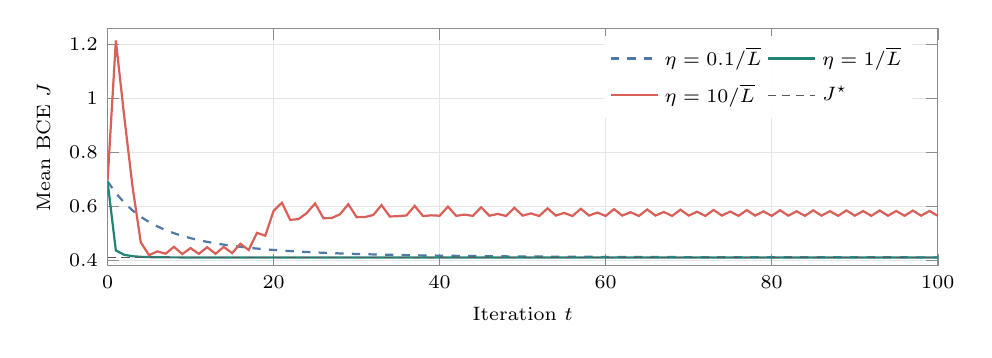
\begin{tikzpicture}
\begin{axis}[
width=\linewidth,height=4.6cm,font=\scriptsize,
tick label style={font=\scriptsize},label style={font=\scriptsize},
axis line style={black!45},tick style={black!45},
grid=major,grid style={black!10},scaled ticks=false,clip=true,
legend style={font=\scriptsize,draw=none,fill=white,fill opacity=.94,
text opacity=1,legend cell align=left,inner sep=2pt,row sep=1pt},
xmin=0,xmax=100,ymin=.38,ymax=1.26,xtick={0,20,40,60,80,100},
ytick={.4,.6,.8,1,1.2},xlabel={Iteration $t$},ylabel={Mean BCE $J$},
legend pos=north east,legend columns=2
]
\addplot[blueplot,dashed,thick,no marks] coordinates {(0,0.69314718056) (1,0.649678680871) (2,0.61439132546) (3,0.585624238094) (4,0.562023339721) (5,0.542515177502) (6,0.526261190705) (7,0.512610131558) (8,0.501056275732) (9,0.491205521341) (10,0.482748994631) (11,0.475442930341) (12,0.469093483976) (13,0.463545300324) (14,0.458672898015) (15,0.454374151035) (16,0.450565329651) (17,0.447177303415) (18,0.444152613702) (19,0.441443200491) (20,0.43900862442) (21,0.436814666315) (22,0.434832216353) (23,0.43303638702) (24,0.431405800148) (25,0.4299220103) (26,0.42856903561) (27,0.427332973879) (28,0.426201686705) (29,0.425164538229) (30,0.424212177975) (31,0.423336359481) (32,0.422529788137) (33,0.421785992964) (34,0.421099218124) (35,0.420464330764) (36,0.419876742429) (37,0.419332341819) (38,0.418827437028) (39,0.4183587058) (40,0.417923152512) (41,0.417518070897) (42,0.417141011622) (43,0.416789754028) (44,0.41646228141) (45,0.416156759367) (46,0.415871516765) (47,0.415605028974) (48,0.415355903072) (49,0.415122864751) (50,0.414904746712) (51,0.414700478347) (52,0.414509076561) (53,0.414329637587) (54,0.414161329664) (55,0.414003386491) (56,0.413855101357) (57,0.413715821863) (58,0.413584945183) (59,0.413461913786) (60,0.413346211578) (61,0.413237360425) (62,0.41313491699) (63,0.413038469883) (64,0.412947637065) (65,0.412862063494) (66,0.412781418984) (67,0.412705396252) (68,0.412633709142) (69,0.412566091002) (70,0.412502293198) (71,0.412442083759) (72,0.412385246137) (73,0.412331578064) (74,0.412280890511) (75,0.412233006727) (76,0.412187761357) (77,0.412144999634) (78,0.412104576627) (79,0.412066356557) (80,0.41203021216) (81,0.411996024102) (82,0.411963680437) (83,0.411933076108) (84,0.411904112482) (85,0.411876696922) (86,0.411850742393) (87,0.411826167088) (88,0.411802894092) (89,0.411780851063) (90,0.411759969936) (91,0.411740186653) (92,0.411721440904) (93,0.411703675895) (94,0.411686838122) (95,0.411670877172) (96,0.411655745526) (97,0.411641398385) (98,0.411627793499) (99,0.411614891015) (100,0.411602653331)};
\addlegendentry{$\eta=0.1/\overline L$}
\addplot[greenplot,thick,no marks] coordinates {(0,0.69314718056) (1,0.437191509981) (2,0.421244533884) (3,0.41587571037) (4,0.413603083544) (5,0.412530660871) (6,0.411991856529) (7,0.411710161675) (8,0.411558899945) (9,0.411476152716) (10,0.411430281998) (11,0.411404607955) (12,0.411390136229) (13,0.411381936122) (14,0.411377271517) (15,0.411374610288) (16,0.411373088664) (17,0.411372217187) (18,0.411371717436) (19,0.411371430579) (20,0.411371265802) (21,0.411371171099) (22,0.411371116646) (23,0.411371085326) (24,0.411371067307) (25,0.411371056939) (26,0.411371050972) (27,0.411371047538) (28,0.411371045561) (29,0.411371044422) (30,0.411371043767) (31,0.41137104339) (32,0.411371043173) (33,0.411371043048) (34,0.411371042976) (35,0.411371042934) (36,0.411371042911) (37,0.411371042897) (38,0.411371042889) (39,0.411371042884) (40,0.411371042882) (41,0.41137104288) (42,0.411371042879) (43,0.411371042879) (44,0.411371042879) (45,0.411371042878) (46,0.411371042878) (47,0.411371042878) (48,0.411371042878) (49,0.411371042878) (50,0.411371042878) (51,0.411371042878) (52,0.411371042878) (53,0.411371042878) (54,0.411371042878) (55,0.411371042878) (56,0.411371042878) (57,0.411371042878) (58,0.411371042878) (59,0.411371042878) (60,0.411371042878) (61,0.411371042878) (62,0.411371042878) (63,0.411371042878) (64,0.411371042878) (65,0.411371042878) (66,0.411371042878) (67,0.411371042878) (68,0.411371042878) (69,0.411371042878) (70,0.411371042878) (71,0.411371042878) (72,0.411371042878) (73,0.411371042878) (74,0.411371042878) (75,0.411371042878) (76,0.411371042878) (77,0.411371042878) (78,0.411371042878) (79,0.411371042878) (80,0.411371042878) (81,0.411371042878) (82,0.411371042878) (83,0.411371042878) (84,0.411371042878) (85,0.411371042878) (86,0.411371042878) (87,0.411371042878) (88,0.411371042878) (89,0.411371042878) (90,0.411371042878) (91,0.411371042878) (92,0.411371042878) (93,0.411371042878) (94,0.411371042878) (95,0.411371042878) (96,0.411371042878) (97,0.411371042878) (98,0.411371042878) (99,0.411371042878) (100,0.411371042878)};
\addlegendentry{$\eta=1/\overline L$}
\addplot[redplot,thick,no marks] coordinates {(0,0.69314718056) (1,1.21428899281) (2,0.935823548177) (3,0.675531835712) (4,0.467498065101) (5,0.419645755461) (6,0.433670240495) (7,0.425220467875) (8,0.450732516522) (9,0.423650304968) (10,0.445951127321) (11,0.424620822585) (12,0.449281616429) (13,0.4246431774) (14,0.450305496584) (15,0.427380441697) (16,0.461967919159) (17,0.439042109382) (18,0.502418713379) (19,0.492197316549) (20,0.583586732482) (21,0.614080872045) (22,0.550550360901) (23,0.553178776262) (24,0.575891812613) (25,0.611396315041) (26,0.556657726962) (27,0.557229711928) (28,0.571211349156) (29,0.608315765108) (30,0.560496159446) (31,0.560905816341) (32,0.568390346216) (33,0.605171423869) (34,0.562913505509) (35,0.564266701734) (36,0.566718163946) (37,0.602169865629) (38,0.56442421925) (39,0.567295306437) (40,0.565752229991) (41,0.599421153316) (42,0.565351409931) (43,0.569978327489) (44,0.565219017748) (45,0.596972370661) (46,0.565901394405) (47,0.57231948985) (48,0.564950001095) (49,0.594832861435) (50,0.566207695697) (51,0.574336537373) (52,0.564840969321) (53,0.592990689552) (54,0.566357763524) (55,0.576055856036) (56,0.564827029818) (57,0.591422759317) (58,0.56640938415) (59,0.577508059268) (60,0.564867513864) (61,0.590100900073) (62,0.566400901773) (63,0.578724933914) (64,0.564936874231) (65,0.588995489683) (66,0.566357711677) (67,0.579737483793) (68,0.565019141355) (69,0.588077581798) (70,0.566296479903) (71,0.580574754395) (72,0.565104490076) (73,0.587320109394) (74,0.566227947552) (75,0.581263192628) (76,0.565187071156) (77,0.58669850708) (78,0.566158830283) (79,0.581826367187) (80,0.565263614561) (81,0.586190963656) (82,0.566093122894) (83,0.582284927533) (84,0.565332514496) (85,0.585778440708) (86,0.5660330024) (87,0.582656715446) (88,0.565393222551) (89,0.585444547518) (90,0.565979454453) (91,0.582956968084) (92,0.56544584254) (93,0.585175333413) (94,0.565932706392) (95,0.583198569541) (96,0.565490859968) (97,0.584959039119) (98,0.565892524075) (99,0.5833923211) (100,0.565528962703)};
\addlegendentry{$\eta=10/\overline L$}
\addplot[black!65,densely dashed,no marks] coordinates {(0,0.411371042878) (100,0.411371042878)};
\addlegendentry{$J^\star$}
\end{axis}
\end{tikzpicture}
\endgroup
